\documentclass[a4paper]{article}
\usepackage[utf8]{inputenc}
\usepackage[spanish, es-tabla, es-noshorthands]{babel}
\usepackage[table,xcdraw]{xcolor}
\usepackage[a4paper, footnotesep = 1cm, width=20cm, top=2.5cm, height=25cm, textwidth=18cm, textheight=25cm]{geometry}
%\geometry{showframe}

\usepackage{tikz}
\usepackage{amsmath}
\usepackage{amsfonts}
\usepackage{amssymb}
\usepackage{float}
\usepackage{graphicx}
\usepackage{caption}
\usepackage{subcaption}
\usepackage{multicol}
\usepackage{multirow}
\setlength{\doublerulesep}{\arrayrulewidth}
\usepackage{booktabs}

\usepackage{hyperref}
\hypersetup{
    colorlinks=true,
    linkcolor=blue,
    filecolor=magenta,      
    urlcolor=blue,
    citecolor=blue,    
}

\newcommand{\quotes}[1]{``#1''}
\usepackage{array}
\newcolumntype{C}[1]{>{\centering\let\newline\\\arraybackslash\hspace{0pt}}m{#1}}
\usepackage[american]{circuitikz}
\usetikzlibrary{calc}
\usepackage{fancyhdr}
\usepackage{units} 

\graphicspath{{../Ejercicio-1/}{../Ejercicio-2/}}

\pagestyle{fancy}
\fancyhf{}
\lhead{22.67 - Señales Aleatorias}
\rhead{Lambertucci, Londero B., Moriconi, Musich, Tolaba}
\rfoot{Página \thepage}

\begin{document}

%%%%%%%%%%%%%%%%%%%%%%%%%
%		Caratula		%
%%%%%%%%%%%%%%%%%%%%%%%%%

\begin{titlepage}
\newcommand{\HRule}{\rule{\linewidth}{0.5mm}}
\center
\mbox{\textsc{\LARGE \bfseries {Instituto Tecnológico de Buenos Aires}}}\\[1.5cm]
\textsc{\Large 22.67 Señales Aleatorias}\\[0.5cm]


\HRule \\[0.6cm]
{ \Huge \bfseries Trabajo práctico N$^{\circ}$3}\\[0.4cm] 
\HRule \\[1.5cm]


{\large

\emph{Grupo 1:}\\
\vspace{3pt}

\begin{tabular}{lr} 	
\textsc{Lambertucci}, Guido Enrique  & 58009 \\
\textsc{Londero Bonaparte}, Tomás Guillermo  & 58150 \\
\textsc{Musich}, Francisco  & 58124\\
\end{tabular}

\vspace{20pt}

\emph{Profesor}\\
\textsc{Hirchoren}, Gustavo Abraham \\
\vspace{3pt}
%\textsc{} \\	

\vspace{100pt}

\begin{tabular}{ll}

Presentado: & 07/02/22\\

\end{tabular}

}

\vfill

\end{titlepage}


%%%%%%%%%%%%%%%%%%%%%
%		Indice		%
%%%%%%%%%%%%%%%%%%%%%

\tableofcontents
\newpage

%%%%%%%%%%%%%%%%%%%%%
%		Informe		%
%%%%%%%%%%%%%%%%%%%%%


\subsection{Introducción}

Se analiza una secuencia $X(n)$ de 32768 muestras, estimando y calculando parámetros de interés, como lo son la autocorrelación, los coeficientes de correlación parcial, a partir de estos se generará un modelo AR con el propósito de ajustar dicha serie, y con los coeficientes autoregresivos diseñar un modelo en variables de estados del sistema para utilizar un filtor de Kalman.\\
A la secuencia se le agregará ruido blanco gaussiano aditivo (AWGN) para simular el ruido de medición.\\
Cabe destacar que en este informe se hará referencia a una variable p, esta tiene un rango entre 1 y 9.\\

\subsection{Estimación de la Autocorrelación} 

Se estiman la autocorrelación mediante el uso de los primeros p elementos de la secuencia brindada. Para ello, se vale del  no polarizados ($R_{np}$) de dicho parámetro. Esta funcion es  empleadas para estimar otras funciones mediante información digitalizada.
\begin{equation}
\begin{gathered}
	R_{np}(k) = \frac{1}{N-k} \sum_{i=0}^{N-k-1} X(i)X(i+k)
\end{gathered}
\end{equation}


\begin{figure}[H]
\centering
	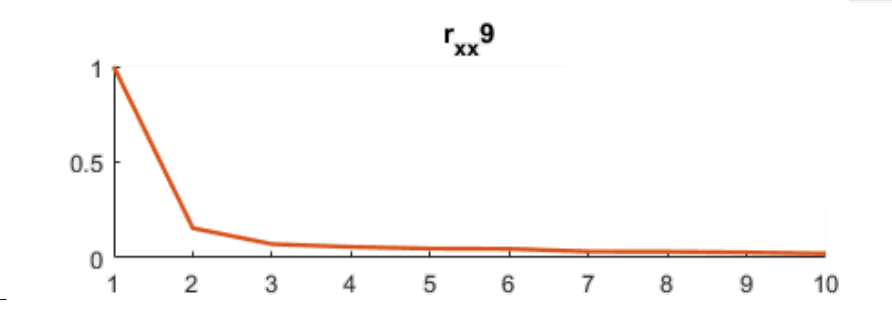
\includegraphics[width=0.8\textwidth, trim = {0 0 0 0},clip]{./Imagenes/correlacion.png}
	\caption{Grafica de los coeficientes de autocorrelación total estimados.}
	\label{fig:rxx}
\end{figure}



\subsection{Coeficientes de correlación parcial}

Con los datos ya extraídos y mediante la resolución de la ecuación de Yule-Walker, fue posible obtener los coeficientes deseados. Esto se realizó con los coeficientes totales obtenidos a través de la estimación no polarizada.
\begin{figure}[H]
\centering
	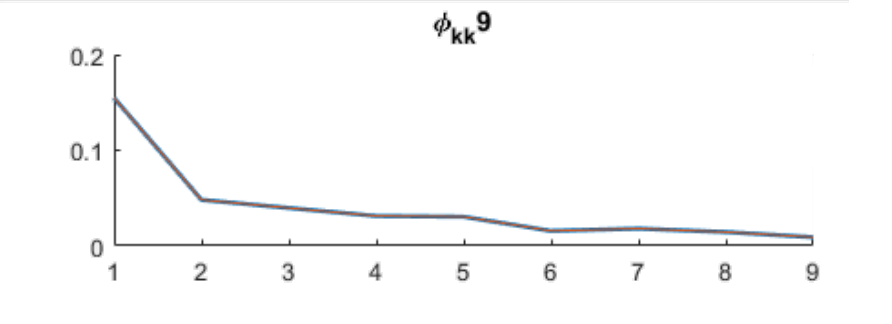
\includegraphics[width=0.7\textwidth, trim = {0 0 0 0},clip]{./Imagenes/phikk.png}
	\caption{Grafica de los coeficientes de autocorrelación parcial obtenidos.}
	\label{fig:phikk}
\end{figure}


\subsection{Modelo del proceso}
\label{subsec:modelo}

El tipo de modelo a utilizar para el proceso será un Auto Regresivo, se utilizará un AR(p).

Para el calculo de los $\phi$, son los obtenidos de la matriz de Yule Walker para cada p.

\subsection{Matrices de la ecuación Yule-Wlaker}
\begin{itemize}

\item Orden 2:
\begin{equation*}
	\phi = 
	\begin{pmatrix}
		0.1473 \\
		0.0481  
	\end{pmatrix}	\	\	\	\
	R =
	\begin{pmatrix}
		1 & 0.1547 \\
		0.1547 & 1					  
	\end{pmatrix}
\end{equation*}

\item Orden 3:
\begin{equation*}
	\phi = 
	\begin{pmatrix}
		0.1454 \\
		0.0423 \\
		0.0396  
	\end{pmatrix}	\	\	\	\
	R =
	\begin{pmatrix}
		1 		& 0.1547 	& 0.0709 \\
		0.1547 	& 1 		& 0.1647 \\
		0.0709 	& 0.1547 	& 1					  
	\end{pmatrix}
\end{equation*}

\item Orden 4:
\begin{equation*}
	\phi = 
	\begin{pmatrix}
		0.1441 \\
		0.0410 \\
		0.0351 \\
		0.0312
	\end{pmatrix}	\	\	\	\
	R =
	\begin{pmatrix}
		1 		& 0.1547 	& 0.0709 	& 0.0564 \\
		0.1547 	& 1 		& 0.1647 	& 0.0709 \\
		0.0709 	& 0.1547 	& 1			& 0.1547 \\
		0.0564	& 0.0709	& 0.1547	& 1		  
	\end{pmatrix}
\end{equation*}

\item Orden 5:
\begin{equation*}
	\phi = 
	\begin{pmatrix}
		0.1432 \\
		0.0399 \\
		0.0338 \\
		0.0268 \\
		0.0304  
	\end{pmatrix}	\	\	\	\
	R =
	\begin{pmatrix}
		1 & 0.1547 & 0.0709 & 0.0564 & 0.0477 \\
    	0.1547 & 1 & 0.1547 & 0.0709 & 0.0564 \\
    	0.0709 & 0.1547 & 1 & 0.1547 & 0.0709 \\
    	0.0564 & 0.0709 & 0.1547 & 1 & 0.1547 \\
    	0.0477 & 0.0564 & 0.0709 & 0.1547 & 1	  
	\end{pmatrix}
\end{equation*}

\item Orden 6:
\begin{equation*}
	\phi = 
	\begin{pmatrix}
		0.1427 \\
		0.0395 \\
		0.0333 \\
		0.0262 \\
		0.0282 \\
		0.0157  
	\end{pmatrix}	\	\	\	\
	R =
	\begin{pmatrix}
		1 & 0.1547 & 0.0709 & 0.0564 & 0.0477 & 0.0461 \\
		0.1547 & 1 & 0.1547 & 0.0709 & 0.0564 & 0.0477 \\
		0.0709 & 0.1547 & 1 & 0.1547 & 0.0709 & 0.0564 \\
		0.0564 & 0.0709 & 0.1547 & 1 & 0.1547 & 0.0709 \\
		0.0477 & 0.0564 & 0.0709 & 0.1547 & 1 & 0.1547 \\
		0.0461 & 0.0477 & 0.0564 & 0.0709 & 0.1547 & 1	
	\end{pmatrix}
\end{equation*}

\item Orden 7:
\begin{equation*}
	\phi = 
	\begin{pmatrix}
		0.1424 \\
		0.0390 \\
		0.0328 \\
		0.0256 \\
		0.0275 \\
		0.0131 \\
		0.0180 
	\end{pmatrix}	\	\	\	\
	R =
	\begin{pmatrix}
	1 & 0.1547 & 0.0709 & 0.0564 & 0.0477 & 0.0461 & 0.0322 \\
	0.1547 & 1 & 0.1547 & 0.0709 & 0.0564 & 0.0477 & 0.0461 \\
	0.0709 & 0.1547 & 1 & 0.1547 & 0.0709 & 0.0564 & 0.0477 \\
	0.0564 & 0.0709 & 0.1547 & 1 & 0.1547 & 0.0709 & 0.0564 \\
	0.0477 & 0.0564 & 0.0709 & 0.1547 & 1 & 0.1547 & 0.0709 \\
	0.0461 & 0.0477 & 0.0564 & 0.0709 & 0.1547 & 1 & 0.1547 \\
	0.0322 & 0.0461 & 0.0477 & 0.0564 & 0.0709 & 0.1547 & 1	  
	\end{pmatrix}
\end{equation*}

\item Orden 8:
\begin{equation*}
	\phi = 
	\begin{pmatrix}
		0.1422 \\
		0.0388 \\
		0.0324 \\
		0.0252 \\
		0.0270 \\
		0.0125 \\
		0.0160 \\
		0.0144  
	\end{pmatrix}	\	\	\	\
	R =
	\begin{pmatrix}	
	1 & 0.1547 & 0.0709 & 0.0564 & 0.0477 & 0.0461 & 0.0322 & 0.0314 \\
	0.1547 & 1 & 0.1547 & 0.0709 & 0.0564 & 0.0477 & 0.0461 & 0.0322 \\
	0.0709 & 0.1547 & 1 & 0.1547 & 0.0709 & 0.0564 & 0.0477 & 0.0461 \\
	0.0564 & 0.0709 & 0.1547 & 1 & 0.1547 & 0.0709 & 0.0564 & 0.0477 \\
	0.0477 & 0.0564 & 0.0709 & 0.1547 & 1 & 0.1547 & 0.0709 & 0.0564 \\
	0.0461 & 0.0477 & 0.0564 & 0.0709 & 0.1547 & 1 & 0.1547 & 0.0709 \\
	0.0322 & 0.0461 & 0.0477 & 0.0564 & 0.0709 & 0.1547 & 1 & 0.1547 \\
	0.0314 & 0.0322 & 0.0461 & 0.0477 & 0.0564 & 0.0709 & 0.1547 & 1					  
	\end{pmatrix}
\end{equation*}

\item Orden 9:
\begin{equation*}
	\phi = 
	\begin{pmatrix}
		0.1420 \\
		0.0386 \\
		0.0323 \\
		0.0250 \\
		0.0268 \\
		0.0122 \\
		0.0156 \\
		0.0132 \\
		0.0090
	\end{pmatrix}	\	\	\	\
	R =
	\begin{pmatrix}	
	1 & 0.1547 & 0.0709 & 0.0564 & 0.0477 & 0.0461 & 0.0322 & 0.0314 & 0.0277 \\
	0.1547 & 1 & 0.1547 & 0.0709 & 0.0564 & 0.0477 & 0.0461 & 0.0322 & 0.0314 \\
	0.0709 & 0.1547 & 1 & 0.1547 & 0.0709 & 0.0564 & 0.0477 & 0.0461 & 0.0322 \\
	0.0564 & 0.0709 & 0.1547 & 1 & 0.1547 & 0.0709 & 0.0564 & 0.0477 & 0.0461 \\
	0.0477 & 0.0564 & 0.0709 & 0.1547 & 1 & 0.1547 & 0.0709 & 0.0564 & 0.0477 \\
	0.0461 & 0.0477 & 0.0564 & 0.0709 & 0.1547 & 1 & 0.1547 & 0.0709 & 0.0564 \\
	0.0322 & 0.0461 & 0.0477 & 0.0564 & 0.0709 & 0.1547 & 1 & 0.1547 & 0.0709 \\
	0.0314 & 0.0322 & 0.0461 & 0.0477 & 0.0564 & 0.0709 & 0.1547 & 1 & 0.1547 \\
	0.0277 & 0.0314 & 0.0322 & 0.0461 & 0.0477 & 0.0564 & 0.0709 & 0.1547 & 1	  
	\end{pmatrix}
\end{equation*}

\end{itemize}

\subsection{Filtro de Kalman}

\subsubsection{Introducción}
En el campo de la estadística y teoría de control, los filtros de Kalman, también conocidos como estimación cuadrática media(LQE), es un algoritmo que utiliza una serie de mediciones realizadas por un observador a través del tiempo, el cual contiene ruido estadístico y otras in-certezas, y  produce estimaciones de variables , que tienden a ser mucho mas acertadas que otras basadas en una única medicion, al estimar la distribución de probabilidad conjunta sobre las variables por cada tiempo $t_k$, El filtro es llamado así por su desarrollador, Rudolf E. Kálmán.
En filtro de Kalman puede ser escrito en una sola ecuación, sin embargo a menudo se conceptualiza como dos fases distintas.

La fase de predicción y la de actualización. La fase de predicción usa la prediccion del estado $k-1$ para producir un estimado del estado actual. Esta prediccion del estado también es conocida como la estimación a-priori y no cuenta con información de la observación actual.  En la fase de actualización la diferencia entre la prediccion a-priori y la observación actual, son muliplicadas por la ganancia de Kalman, y combinada con la última estimación, para mejorarla, esto es conocido como el estimador a-posteriori.

Estas dos etapas se van turnando usualmente.\\


\subsubsection{Modelo en variables de estado}
Para el modelo en variables de estado, se tuvieron en cuenta las siguientes matrices:
\begin{itemize}
\item La matriz $\Phi$ también conocida como la matriz de transición de estados está construida de la siguiente manera: la primera fila son los coeficientes del modelo autoregresivo, mientras que para el resto es la identidad.
\item La matriz $H$ también conocida como el modelo de observación es una matriz nula excepto en la posición (0,0) donde vale 1.
\item Q es la matriz de covarianza de ruido del proceso: Es una matriz cuadrada de p x p  donde el termino [0,0] es el ruido del proceso.
\item R es la matriz de covarianza de ruido de observación: es una matriz cuadrada de p x p diagonal con valor $\sigma_v^2$
\end{itemize}
\begin{figure}[H]
\centering
	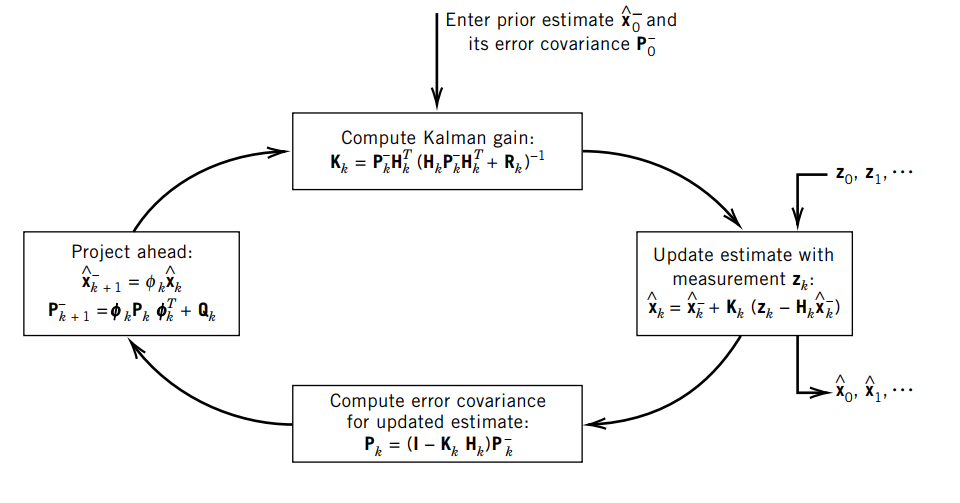
\includegraphics[width=0.7\textwidth, trim = {0 0 0 0},clip]{./Imagenes/kalman_loop.png}
	\caption{Ciclo del filtro de Kalman.}
	\label{fig:kalmanfilter}
\end{figure}


\subsubsection{Implementacion del filtro recursivo}
En la implementación del filtro se utilizó las variables de estado detalladas en la anterior sección.

En el caso del trabajo práctico se generó una secuencia  $v_k$ de ruido blanco y gaussiano con varianza R=$\sigma_v^2$ y se sumó a la secuencia $x_k$. Y a esto se le aplicó el filtro de kalman, finalmente se hizo lo mismo pero variado el valor de $\sigma_v^2$.


\subsection{Análisis de resultados}
A continuación se observan la señal de entrada, la señal medida y la de saldia del filtro..

Aquí se observa como es la relación señal a ruido sin la utilización del filtro de Kalman, y por otro lado su mejora al utilizarlo.

\begin{figure}[H]
\centering
	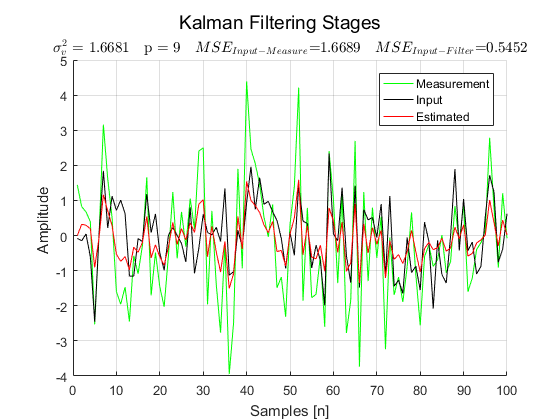
\includegraphics[width=0.7\textwidth, trim = {0 0 0 0},clip]{./Imagenes/Kalman_Filter.png}
	\caption{Comparación de entrada, medición y predicción del sistema.}
	\label{fig:kalmanfilter}
\end{figure}


Además se varió el valor del $\sigma_v^2$ entre 0.01 $\sim$ 100 y se observó la gran mejora porcentual del MSE en función del sigma, viendo que cuanto mayor es la varianza mayor es la mejora porcentual 
\begin{figure}[H]
\centering
	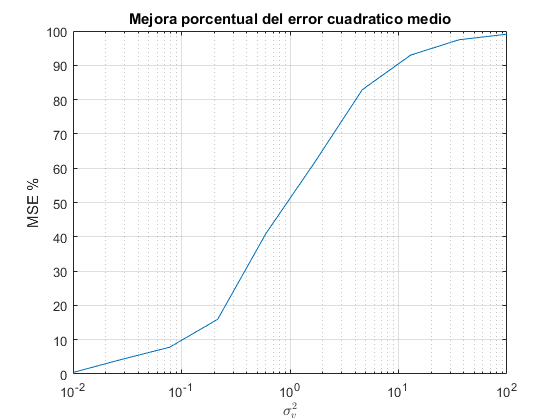
\includegraphics[width=0.7\textwidth, trim = {0 0 0 0},clip]{./Imagenes/Error_porcentual.png}
	\caption{Variación del error porcentual en función de la varianza.}
	\label{fig:errorporcent}
\end{figure}
\subsection{Conclusiones}
Se observó como la utilización de un filtro de Kalman reduce significativamente el MSE en un entorno ruidoso. Una herramienta sumamente útil múltiples campos. Definitvamente en entornos donde se trata con mediciones del mundo físico el cual está sumido en ruidos.
Al ser un filtro recursivo permite una mayor velocidad de computo que algunos que no lo son debido a que no debe tener una memoria tan grande.

\subsection{Código implementado}
A continuación se muestra todo el código utilizado en el proyecto.
\begin{itemize}
\item Main.m:
	\lstinputlisting[language=Matlab]{../Matlab/Main.m}
	
\item Cpar.m:
	\lstinputlisting[language=Matlab]{../Matlab/cpar.m}
	
\item Rnp.m:
	\lstinputlisting[language=Matlab]{../Matlab/Rnp.m}
	
\item kalman.m:
	\lstinputlisting[language=Matlab]{../Matlab/kalman.m}

\end{itemize}

\end{document}